\documentclass{standalone}

\RequirePackage{fix-cm}
\usepackage{fontspec}
\newfontfamily\fontused{Arial}

\usepackage{tikz}
\definecolor{xred}{HTML}{FF3838}
\definecolor{xblue}{HTML}{3778FF}
\definecolor{xyellow}{HTML}{FFF82F}

\begin{document}
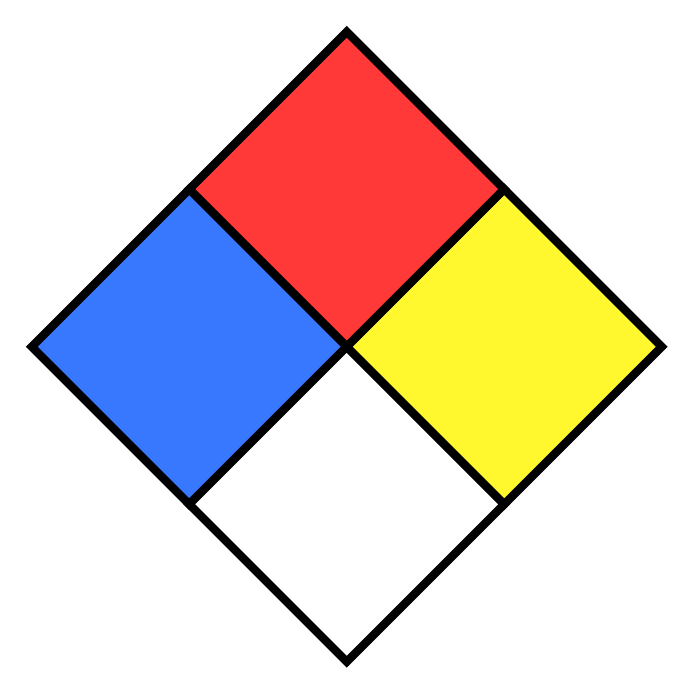
\begin{tikzpicture}
	\tikzset{
		diamond/.style={line width=3pt, fill=#1},
		every node/.style={font=\fontused\fontsize{70pt}{70pt}\selectfont\bfseries, align=center, anchor=center},
	}

	\draw[diamond={xred}] (6,10) -- (4,8) -- (6,6) -- (8,8) -- cycle;
	\draw[diamond={xblue}] (4,8) -- (2,6) -- (4,4) -- (6,6) -- cycle;
	\draw[diamond={white}] (6,6) -- (4,4) -- (6,2) -- (8,4) -- cycle;
	\draw[diamond={xyellow}] (8,8) -- (6,6) -- (8,4) -- (10,6) -- cycle;

	\node[] at (6,8) {\fire};
	\node[] at (4,6) {\health};
	\node[] at (6,4) {\extra};
	\node[] at (8,6) {\react};
\end{tikzpicture}
\end{document}
